\subsection{The Logic Trap: A Trick From Cantor’s Playbook}

To understand Gödel’s method, we need to rewind to an earlier genius move: \textbf{Cantor’s diagonalization argument}.

Cantor used this technique to show that the real numbers are \emph{uncountably infinite} — that is, there are more real numbers than there are natural numbers. He imagined listing every real number between 0 and 1, then cleverly constructing a new number by changing the $n$-th digit of the $n$-th number in the list. This new number couldn’t be on the list — it differed from every number in at least one digit. \textbf{Conclusion:} No list of all real numbers can ever be complete.

\begin{quote}
Gödel applied Cantor's diagonal argument... to \textbf{mathematical statements}.
\end{quote}

Here’s the (slightly simplified) gist.

\subsubsection{Enumerate Everything} 

Gödel’s first move was deceptively simple but deeply clever: turn language into numbers. Every symbol, formula, and proof in mathematics was given a unique number, like assigning a barcode to every idea. This wasn't just for bookkeeping—it was a conceptual bridge. 

\begin{quote}
Suddenly, statements about math \emph{became} math. 
\end{quote}

Proofs could be studied like numbers. Reason itself could be encoded, manipulated, and—crucially—referred to. What had once been a realm of abstract thought now had a digital backbone. Logic got a ZIP code.


\vspace{1em}

\begin{figure}[H]
\centering
\begin{tikzpicture}[
  every node/.style={font=\small},
  box/.style={draw, minimum height=0.8cm, minimum width=0.8cm, rounded corners, fill=gray!5},
  arrow/.style={->, thick},
  symbol/.style={font=\small\ttfamily},
  number/.style={font=\small\ttfamily\bfseries}
]

% --- Symbol nodes ---
\matrix (symbols) [row sep=1.0cm, column sep=0.2cm, matrix of nodes, nodes={box}] {
  \texttt{$\forall$} & \texttt{x} & \texttt{(} & \texttt{P} & \texttt{(} & \texttt{x} & \texttt{)} & \texttt{->} & \texttt{Q} & \texttt{(} & \texttt{x} & \texttt{)} & \texttt{)} \\
};

% --- Number nodes ---
\matrix (numbers) [below=1.6cm of symbols, matrix of nodes, column sep=0.3cm, nodes={number}] {
  1 & 24 & 5 & 16 & 5 & 24 & 6 & 2 & 17 & 5 & 24 & 6 & 7 \\
};

% --- Labels ---
\node[above=1.2cm of symbols-1-1, anchor=west, font=\small\bfseries] at (symbols-1-1.west) 
  {Statement: $\forall x(P(x) -> Q(x))$ };

\node[below=0.6cm of numbers-1-1, anchor=west, font=\small\itshape] at (numbers-1-1.west)
  {Each symbol is assigned a unique Gödel number.};

% --- Arrows from symbols to numbers ---
\foreach \i in {1,...,13} {
  \draw[arrow, gray] (symbols-1-\i.south) -- (numbers-1-\i.north);
}

\end{tikzpicture}
\caption{Gödel numbering: assigning unique numbers to each symbol in a formula to encode it arithmetically.}
\end{figure}

\vspace{1em}
    
\subsubsection{Create Paradox} 

Here's where Gödel pulled off something wild. He didn't just encode math into numbers—he encoded logic itself into arithmetic. And then, like a master of linguistic judo, he used the system's own language to bend it back on itself.

He constructed a statement \( G \) that talks about its own provability. Not with hand-wavy metaphysics, but with cold, hard symbols and code. Through a meticulous process of encoding, substitution, and fixed points, he crafted a sentence that effectively says:

\[
G = \text{“This statement cannot be proven in this system.”}
\]

It's a kind of mathematical snake eating its tail—a sentence that, through arithmetic, refers to itself. Not by name, but by number. It doesn’t shout its identity; it whispers it through the structure of the system.

This wasn’t the first time someone flirted with self-reference. 

\begin{quote}
The liar paradox—“This sentence is false”—goes back to the ancients. But Gödel translated that paradox into the formal language of mathematics. 
\end{quote}

He built a sentence so precise, so syntactically valid, that it passed all the checks of formal logic—yet still managed to say something no system could comfortably admit. This is the move that cracks the foundation.
    
\vspace{1em}

\begin{figure}[H]
\centering
\begin{tikzpicture}[
  every node/.style={font=\small},
  box/.style={draw, rounded corners, fill=gray!10, minimum width=2.5cm, minimum height=1.4cm},
  arrow/.style={->, thick},
  text width=3cm,
  align=center
]

% Statement G
\node[box] (G) at (0,0) 
  {Statement $G$: \\
   \textit{“This statement cannot be proven in this system.”}};

% Gödel Encoding box
\node[box, minimum width=2.8cm, minimum height=1cm, fill=blue!10] (code) at (0,-2.2) 
  {Gödel number of $G$};

% Arrow from G to its Gödel number
\draw[arrow] (G.south) -- (code.north) node[midway, right, font=\scriptsize] {encoding};

% Curved arrow from Gödel number to the statement (self-reference)
\draw[arrow, bend left=40, red!70!black] (code.west) to node[midway, above, font=\scriptsize] {references itself} (G.west);

% Reflection metaphor (mirror box)
\node[box, fill=gray!5, minimum width=2.2cm] (mirror) at (4,0) {Mirror};

% Arrow to the west anchor of the mirror box
\draw[->, thick, dashed, gray] (G.east) -- (mirror.west);

% Caption
\node[below=1.2cm of code, text width=10cm, align=center, font=\footnotesize\itshape] 
  {Gödel's trick: encode a sentence that refers to its own Gödel number and asserts that it cannot be proven. A paradox of arithmetic born from arithmetic.};

\end{tikzpicture}
\caption{Gödel’s statement $G$ encodes its own unprovability by referencing its Gödel number.}
\end{figure}

\vspace{1em}


\subsubsection{Prove Paradox} 

Now the paradox hits. Suppose the formal system—our proud, consistent edifice of logic—manages to prove the statement \( G \). But recall what \( G \) actually says: “This statement cannot be proven in this system.” If the system does prove it, then \( G \) is false, because it claimed it was unprovable. That’s not just a little contradiction—it’s a full-blown logical meltdown. The system has just proven a falsehood. 

This isn’t like a bad answer on a math test—it’s structural rot in the foundation of mathematics. It means the system is \emph{inconsistent}—capable of proving things that aren’t true. And in formal logic, once inconsistency sets in, anything can be proven. If \( 0 = 1 \), then every statement becomes trivially true. Logic collapses into noise.

\begin{quote}
If the system \emph{can} prove \( G \), it destroys itself. 
\end{quote}

That’s not just a bug; it’s a paradox by design. Gödel built a sentence that acts like a mirror held up to the system—a mirror that cracks if the system dares to accept the reflection as valid.



\vspace{1em}

\begin{figure}[H]
\centering
\begin{tikzpicture}[
  every node/.style={font=\small},
  box/.style={draw, minimum width=2.6cm, minimum height=1.1cm, rounded corners=3pt, fill=gray!5},
  arrow/.style={->, thick},
  condition/.style={draw, ellipse, minimum height=1cm, minimum width=2.4cm, fill=orange!10}
]

% System box
\node[box] (system) at (0,0) {Assume: System can prove $G$};

% Statement box
\node[box] (statement) at (5,0) {Then $G$ is true};

% Arrow between them
\draw[arrow] (system) -- node[above] {Proof} (statement);

% Implication box
\node[condition] (contradiction) at (2.5,-2.2) {But $G$ says it can't be proven};

\draw[arrow] (statement) -- (contradiction);
\draw[arrow, dashed, red] (contradiction.south) -- ++(0,-1) node[below, align=center] {\textbf{Contradiction:}  System proves falsehood};

\end{tikzpicture}
\caption{The paradox of \( G \): If the system proves it, then it is false — implying inconsistency.}
\end{figure}

\vspace{1em}


\subsubsection{QED} 

But here's the twist. If the system \emph{can’t} prove \( G \), then paradoxically... \( G \) is true. Why? Because all it's doing is stating a fact about itself—that it cannot be proven. And if no proof exists for \( G \), well, that’s exactly what \( G \) claimed all along.

\begin{quote}
\( G \) is \emph{true but unprovable}. 
\end{quote}

\( G \) is a sentence that accurately describes its own unprovability. It is like a ghost slipping through the walls of logic, it exists, it speaks, but no system can pin it down. This isn’t just a clever riddle. It’s a philosophical uppercut.

Gödel didn’t just prove a technical lemma—he shattered a century of foundational dreams. Hilbert had hoped for a machine-proof universe, one where every truth could be formalized, deduced, and verified. Gödel showed that any system strong enough to express arithmetic will necessarily contain truths that lie beyond its reach.

It’s like discovering that no matter how perfect your map, there will always be territory it cannot chart. \( G \) is the forbidden island, the off-grid reality that resists formalization. It echoes Cantor’s diagonal argument, where the list of all real numbers always misses one just beyond its grasp. Only this time, the missing number isn’t mathematical: it’s epistemological.

This is why Gödel’s theorem hits so hard. It reveals a fundamental asymmetry between truth and proof; between what is, and what can be demonstrated; between what exists in the universe of meaning, and what the machinery of logic can ever hope to certify.

\vspace{1em}

\begin{figure}[H]
\centering
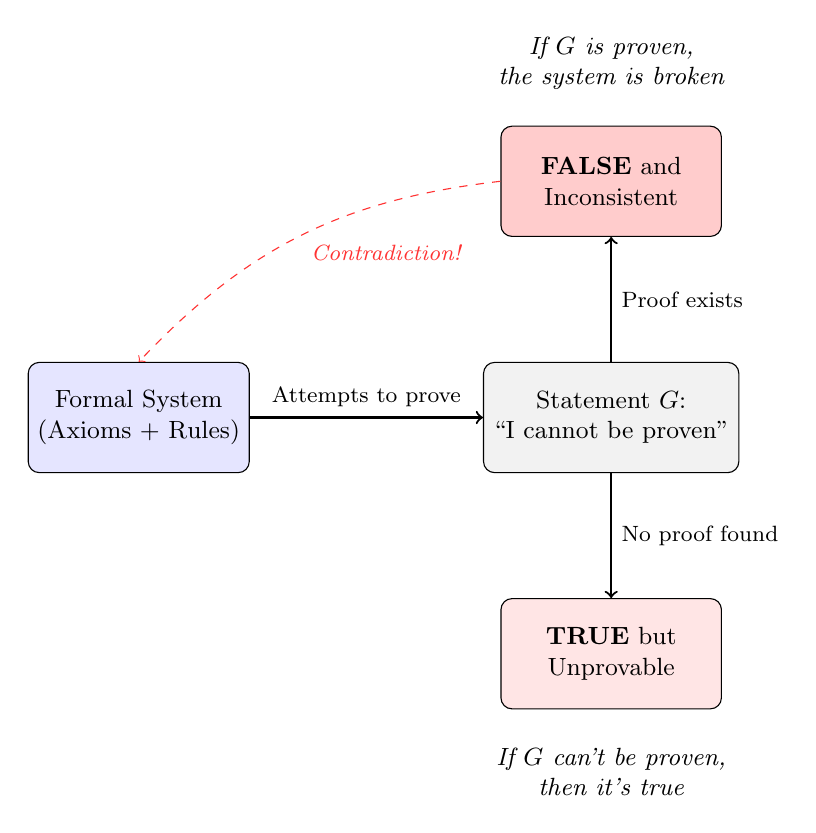
\begin{tikzpicture}[
  every node/.style={font=\small},
  box/.style={draw, rounded corners, minimum width=2.8cm, minimum height=1.4cm, align=center},
  arrow/.style={->, thick}
]

% Nodes
\node[box, fill=blue!10] (system) at (0, 0) {Formal System\\(Axioms + Rules)};
\node[box, fill=gray!10] (G) at (6, 0) {Statement $G$:\\``I cannot be proven''};
\node[box, fill=red!10] (true) at (6, -3) {\textbf{TRUE} but \\ Unprovable};
\node[box, fill=red!20] (false) at (6, 3) {\textbf{FALSE} and\\ Inconsistent};

% Arrows
\draw[->, thick] (system.east) -- node[above] {\footnotesize Attempts to prove} (G.west);
\draw[->, thick] (G.south) -- node[right] {\footnotesize No proof found} (true.north);
\draw[->, thick] (G.north) -- node[right] {\footnotesize Proof exists} (false.south);

% Annotations
\node[align=center, font=\small\itshape] at (6, -4.5) {If $G$ can't be proven, \\ then it's true};
\node[align=center, font=\small\itshape] at (6, 4.5) {If $G$ is proven, \\ the system is broken};

% Optional arrows showing paradox
\draw[->, dashed, red!80] (false.west) to[bend left=-20] node[below right, font=\footnotesize\itshape] {Contradiction!} (system.north);

\end{tikzpicture}
\caption{Gödel’s paradox: $G$ creates a loop where proving it breaks the system, and failing to prove it makes it true.}
\end{figure}

\vspace{1em}



\begin{tcolorbox}[title={\textbf{Historical Sidebar: No Soul in the Cogs — Leibniz’s Mill Argument}}, colback=gray!5, colframe=black, fonttitle=\bfseries]

  In his \textit{Monadology} and other late writings, \textbf{Gottfried Wilhelm Leibniz} offered one of the earliest and most elegant critiques of materialism in the philosophy of mind—a thought experiment now known as the \textbf{Mill Argument}.
  
  Leibniz imagined a hypothetical machine that could think, perceive, and feel. Now suppose we could enlarge this machine and walk around inside it, like a 17th-century tour through a windmill powered by divine doubt. What would we see? Nothing but gears grinding and parts colliding. But nowhere—not behind a gear, not under a crank—would we find \textit{perception} itself. The ghost in the machine, it seems, doesn’t clock in for the tour.
  
  His conclusion? You don’t get a mind by assembling matter, no matter how clever the arrangement. Consciousness, for Leibniz, belongs to \textbf{monads}: indivisible, non-material entities with inner lives. Their coordination isn’t mechanical, but metaphysical—arranged by a pre-established harmony.
  
  Centuries later, this rejection of mechanistic reductionism echoed in the work of \textbf{Kurt Gödel}. Like Leibniz, Gödel believed that the mind reaches truths no machine could ever grind out. His incompleteness theorems weren’t just mathematical curiosities—they were metaphysical statements: the soul can’t be simulated. For Gödel, as for Leibniz, there is indeed no soul in the cogs.
\end{tcolorbox}










